\documentclass[12pt]{article}

% Language setting
% Replace `english' with e.g. `spanish' to change the document language
\usepackage[english]{babel}

% Set page size and margins
% Replace `letterpaper' with `a4paper' for UK/EU standard size
\usepackage[a4paper,top=2cm,bottom=2cm,left=3cm,right=3cm,marginparwidth=1.75cm]{geometry}

% Useful packages
\usepackage{amsmath,amssymb,amsthm}
\newtheorem*{defn}{Definition}
\newtheorem*{exmp}{Example}
\newtheorem*{lem}{Lemma}
\newtheorem*{prob}{Problem}
\usepackage{graphicx}
\usepackage{multicol}
\usepackage{savetrees}
\usepackage{txfonts}
\usepackage{tabularx}
\usepackage{tabularray}
\usepackage{framed}
\usepackage{titlesec}
\titleformat{\section}{\Large\bfseries}{\thesection}{1em}{}
\titleformat{\subsection}{\large\bfseries}{\thesubsection}{1em}{}
\titleformat{\subsubsection}{\large\bfseries}{\thesubsubsection}{1em}{}
\usepackage{float}
\usepackage{tikz}
\usepackage{pgfgantt}
\usepackage{subcaption}
\usepackage{xcolor}
\usepackage{contour}
\usepackage{ulem}
\usepackage[colorlinks=true, allcolors=blue]{hyperref}
\usepackage{pdfpages}
\usepackage{pdflscape}
\usepackage{parskip}
\usepackage{multirow}
\usepackage{colortbl}
\usepackage{listings}

% Make sections bigger, bold, and with more spacing
\titleformat{\section}
  {\Huge\bfseries} % Larger font size and bold
  {\thesection}     % Section number
  {1em}             % Horizontal spacing between number and title
  {}                % Code before title
  [\vspace{1ex}]    % Increase space after section

% Make subsections bigger and bold
\titleformat{\subsection}
  {\LARGE\bfseries} % Larger font size and bold
  {\thesubsection}  % Subsection number
  {1em}             % Horizontal spacing between number and title
  {}                % Code before title
  [\vspace{0.5ex}]  % Increase space after subsection
% Make subsubsections bigger and bold
\titleformat{\subsubsection}
  {\Large\bfseries} % Larger font size and bold
  {\hspace{2em}\thesubsubsection}  % Subsection number
  {1em}             % Horizontal spacing between number and title
  {}                % Code before title
  [\vspace{0.5ex}]  % Increase space after subsection



\titlespacing*{\section}{0pt}{3.5ex}{0ex}
\titlespacing*{\subsection}{0pt}{1.5ex plus 1ex minus 0.5ex}{1ex plus 0.5ex minus 0.2ex}


\newcommand{\smalltitle}[1]{%
    \par\vspace{0.5\baselineskip} % Add space above the title
    \noindent\hspace{2em}\textbf{\large #1}\par % Indented title formatting
    \vspace{0.5\baselineskip} % Add space below the title
}
\newcommand{\smallsmalltitle}[1]{%
    \par\vspace{0.5\baselineskip} % Add space above the title
    \noindent\textbf{#1}\par % Indented title formatting
    \vspace{0.5\baselineskip} % Add space below the title
}

\renewcommand{\ULdepth}{1.8pt}
\contourlength{0.8pt}


\newcommand{\myuline}[1]{
  \uline{\phantom{#1}}%
  \llap{\contour{white}{#1}}%
}

\newcommand{\textbu}[1]{
    \myuline{\textbf{#1}}
}

%%%% LISTINGS %%%%

\definecolor{deepblue}{rgb}{0,0,0.5}
\definecolor{deepred}{rgb}{0.6,0,0}
\definecolor{deepgreen}{rgb}{0,0.5,0}
\definecolor{deepgrey}{rgb}{0.25,0.25,0.25}
\definecolor{lightgrey}{rgb}{0.8,0.8,0.8}
\definecolor{orange}{rgb}{0.8,0.55,0.41}
\definecolor{orangekeywords}{rgb}{0.8,0.4,0}


% AMPL style for highlighting

\lstdefinelanguage{ampl}
{
keywords={},
}


\newcommand\amplstyle{\lstset{
language=ampl,
backgroundcolor=\color{white},
basicstyle=\scriptsize\ttfamily,
numbers=left,
emph={subject to, minimize, reset},          % Custom highlighting
morekeywords={set,param,var,arc,integer,minimize,maximize,subject,to,node,sum,in,Current,complements,integer,solve_result_num,IN,contains,less,suffix,INOUT,default,logical,sum,Infinity,dimen,max,symbolic
,Initial,div,min,table,LOCAL,else,option,then,OUT,environ,setof     ,union,all,exists,shell_exitcodeuntil,binary,forall,solve_exitcodewhile     ,by,if,solve_messagewithin,check,in,solve_result},             % Add keywords here
keywordstyle=\bfseries\color{deepblue},
emphstyle=\bfseries\color{deepred},    % Custom highlighting style
morestring=[b]",
stringstyle=\color{deepblue},
commentstyle=\color{deepgreen},
comment=[l]{\#},
frame=single,                         % Any extra options here
showstringspaces=false            % 
}}


% AMPL environment
\lstnewenvironment{ampl}[1][]
{
\amplstyle
\lstset{#1}
}
{}

% AMPL for external files
\newcommand\amplexternal[2][]{{
\amplstyle
\lstinputlisting[#1]{#2}}}

% AMPL for inline
\newcommand\amplinline[1]{{\amplstyle\lstinline!#1!}}

\lstset{
    language=Python,
    basicstyle=\scriptsize\ttfamily,
    numbers=left,
    numbersep=5pt,
    frame=single,
    breaklines=true,
    breakatwhitespace=true,
    showstringspaces=false,
    tabsize=4,
    captionpos=b,
    morekeywords={as},
    keywordstyle=\bfseries\color{orangekeywords},    % Custom highlighting style
    stringstyle=\color{deepblue},
    commentstyle=\color{deepgreen},
}

%%%% End of LISTINGS %%%%


\title{GEP submission 2}
\author{Zephyr Serret Verbist}

\begin{document}

\begin{titlepage}

\includepdf[]{portada_followup.pdf}
\end{titlepage}

\renewcommand*\contentsname{Table of contents}
\tableofcontents
\listoffigures
\listoftables
\newpage



\section{Introduction and contextualization}\label{sec:context}
This article provides context for the research conducted in Zephyr Serret Verbist's Bachelor's Thesis, undertaken at the Faculty of Informatics of Barcelona (FIB) at the Universitat Politècnica de Catalunya, under the guidance of Gabriel Valiente Feruglio. It encompasses an exploration of the research's background, the applied methodology, the rationale behind the study, and the obtained results.

\subsection{Terms and concepts used in this study}

\subsubsection{Hypergraphs}

Hypergraphs are an extension of graphs that employs hyperedges instead of edges. A hyperedge is defined by two non-empty sets of nodes: a tail set and a head set. The hyperedge models a relationship originating from all elements in its tail set to all elements in its head set, or it can be undirected.

Let us recall from~\cite{Gallo.Longo.Pallottino.Nguyen:1993} the following definition, where we impose the tail and head of a hyperedge to be nonempty sets of nodes.

\begin{defn}
A directed hypergraph $H=(V,E)$ consists of a set of nodes $V$ and a set of hyperedges $E=\{\ (T(e),H(e))\ \mid T(e)\ \subseteq\ V,\ H(e)\ \subseteq\ V,\ T(e)\neq\emptyset,\ H(e)\neq\emptyset\}$.
\end{defn}

\begin{figure}[H]
\centering
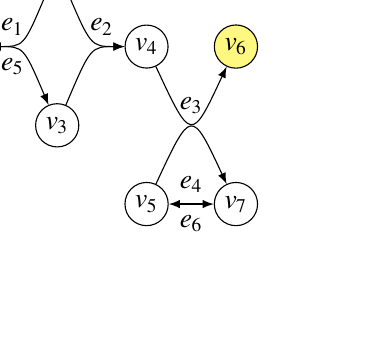
\begin{tikzpicture}[baseline,xscale=0.5675]
    \tikzstyle{every picture}=[thick]
    \tikzstyle{every node}=[inner sep=2pt,circle,draw]
    \draw (0,2) node (1) {$v_1$};
    \draw (2,3) node (2) {$v_2$};
    \draw (2,1) node (3) {$v_3$};
    \draw (4,2) node (4) {$v_4$};
    \draw (4,0) node (5) {$v_5$};
    \draw (6,2) node [fill=yellow!50] (6) {$v_6$};
    \draw (6,0) node (7) {$v_7$};
    \draw[latex-latex] (1) .. controls (1.25,2) .. (2);
    \draw[latex-latex] (1) .. controls (1.25,2) .. (3);
    \draw[-latex] (2) .. controls (2.75,2) .. (4);
    \draw[-latex] (3) .. controls (2.75,2) .. (4);
    \draw[-latex] (4) .. controls (5,0.78125) .. (6);
    \draw[-latex] (5) .. controls (5,1.21875) .. (7);
    \draw[latex-latex] (5) -- (7);
    \draw (1,2.25) node[draw=none] {$e_1$};
    \draw (3,2.25) node[draw=none] {$e_2$};
    \draw (5,1.25) node[draw=none] {$e_3$};
    \draw (5,0.25) node[draw=none] {$e_4$};
    \draw (1,1.75) node[draw=none] {$e_5$};
    \draw (5,-0.25) node[draw=none] {$e_6$};
\end{tikzpicture}
\caption[Example of a directed hypergraph $H=(V,E)$]
%{\tabular[t]{@{}l@{}}Example of a directed hypergraph $H=(V,E)$\\ with $V=\{v_1,v_2,v_3,v_4,v_5,v_6,v_7\}$ and $E=\{e_1,e_2,e_3,e_4,e_5,e_6\}$\\ where $e_1=(\{v_1\},\{v_2,v_3\})$, $e_2=(\{v_2,v_3\},\{v_4\})$, $e_3=(\{v_4,v_5\},\{v_6,v_7\})$,\\\hspace{24pt} $e_4=(\{v_5\},\{v_7\})$, $e_5=(\{v_2,v_3\},\{v_1\})$, $e_6=(\{v_7\},\{v_5\})$.\endtabular}
{Example of a directed hypergraph $H=(V,E)$ with $V=\{v_1,v_2,v_3,v_4,v_5,v_6,v_7\}$ and $E=\{e_1,e_2,e_3,e_4,e_5,e_6\}$, where $e_1=(\{v_1\},\{v_2,v_3\})$, $e_2=(\{v_2,v_3\},\{v_4\})$, $e_3=(\{v_4,v_5\},\{v_6,v_7\})$, $e_4=(\{v_5\},\{v_7\})$, $e_5=(\{v_2,v_3\},\{v_1\})$, $e_6=(\{v_7\},\{v_5\})$.}
\label{fig:Hypergraph-example}
\end{figure}

\subsubsection{Metabolic Pathway}
A metabolic pathway is a set of linked chemical reactions that occur in the cell.
Hypergraphs are particularly well-suited for modeling metabolic pathways because metabolic reactions often involve multiple substrates and multiple products~\cite{Pearcy.Crofts.Chuzhanova:2014}. While these reactions typically have a dominant direction, it is also possible for some reactions to proceed in the opposite direction~\cite{SORRIBAS1989239}. Figure \ref{fig:hsa00600} shows a representation of the Sphingolipid metabolic pathway map in Homo Sapiens.

\begin{figure}[H]
    \centering
    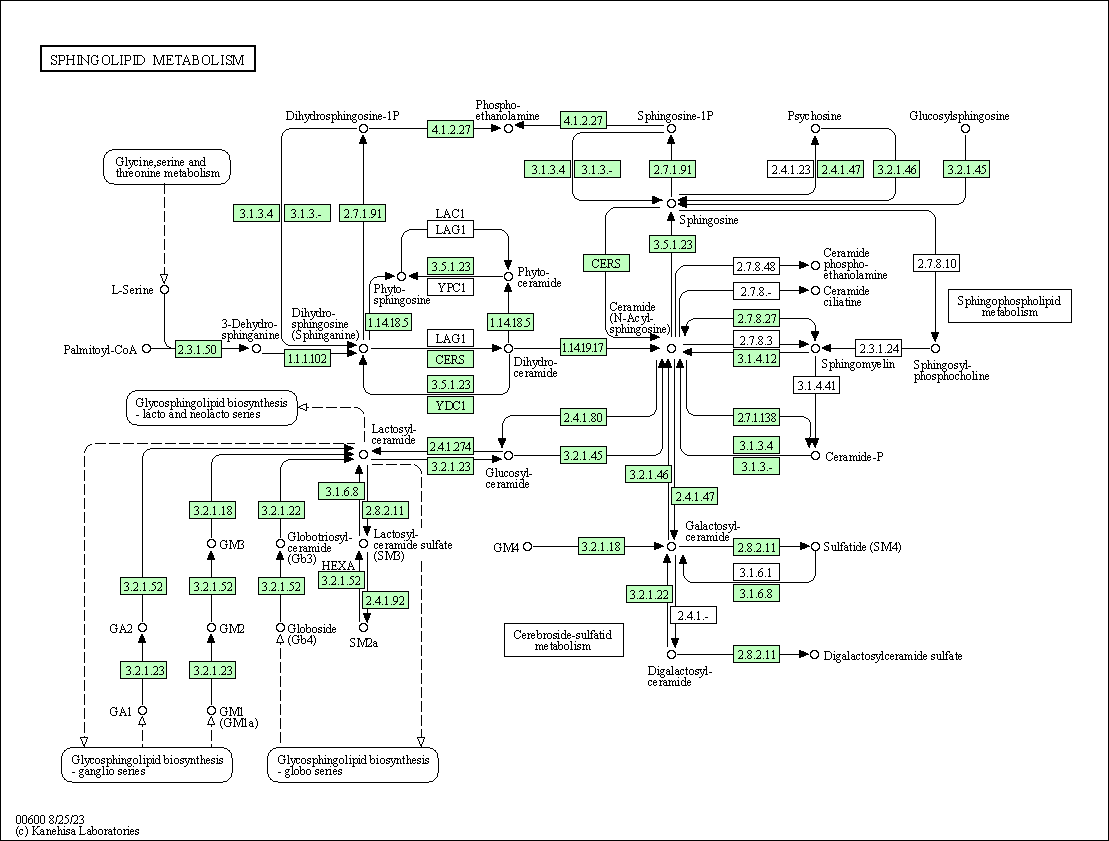
\includegraphics[width=\textwidth]{GEP1/hsa00600.png}
    \caption{Sphingolipid metabolism. Source: \href{https://www.kegg.jp/entry/map00600}{KEGG entry hsa map00600}}
    \label{fig:hsa00600}
\end{figure}

Throughout this study, we will utilize authentic metabolic pathways sourced from the Kyoto Encyclopedia of Genes and Genomes (KEGG) database. These real-world pathways will serve a dual purpose: firstly, to rigorously assess the effectiveness of our proposed solution, and secondly, to establish a robust benchmark against which future evaluations can be conducted. The determination of practical relevance and application of our results will be subject to evaluation by researchers in the field, ensuring the impartial assessment of our methodology within the context of real biological systems.

Using hypergraphs to model metabolic pathways allows us to capture the complexity and interdependencies inherent in cellular metabolism. This modeling approach provides a robust framework for studying and analyzing the intricate network of biochemical reactions that occur within cells, shedding light on the underlying processes crucial to understanding cellular function and regulation.

\subsubsection{Internal and external vertices} \label{sec:internal_external_definition}
In the context of directed graphs and hypergraphs, we introduce the concept of internal and external nodes. An internal node is defined by meeting two essential criteria: it must have an in-degree greater than zero, indicating incoming connections, and it must also have an out-degree greater than zero, signifying outgoing connections. Conversely, if a node fails to satisfy either of these criteria, it is considered external.

Applying this concept to a given metabolic pathway and its corresponding hypergraph, an internal node implies that the associated metabolite serves as both a substrate and a product within the metabolic pathway. In contrast, when a node is external, it indicates that the metabolite functions either as an input into the metabolic pathway or as a final product, thereby shedding light on the role of the metabolite in the broader context of the pathway's inputs and outputs.

\subsection{Problem definition}

In the context of undirected or partially directed hypergraphs, the objective is to determine an optimal orientation of the hyperedges that minimizes the number of external nodes. An external node is defined as a node within the hypergraph that lacks either incoming or outgoing hyperedges. To address this problem, we aim to develop an integer linear programming (ILP) model capable of finding a feasible solution within a reasonable computational timeframe.

In essence, this problem seeks to find an orientation for the hyperedges that maximizes the internal connectivity of nodes while minimizing their isolation as external nodes. The ILP model will serve as a valuable tool to achieve this goal, providing an efficient means of optimizing the orientation of hyperedges and facilitating the analysis of complex hypergraph structures.

\subsection{Stakeholders}

In this research project, the primary stakeholders involved are as follows:
\begin{list}{}{\leftmargin=0em}
\item \textbf{Thesis Supervisor and Team}: The thesis supervisor and their team play a pivotal role as stakeholders in this endeavor, and they are poised to benefit significantly from the study's success. Their guidance, mentorship, and valuable insights contribute significantly to the project's progress. Moreover, their team, concurrently tackling a similar problem, presents opportunities for collaboration and knowledge sharing that enrich our collective efforts. The success of this research not only advances our academic pursuits but also enhances the knowledge and expertise of our thesis supervisor and their team, positioning them at the forefront of cutting-edge research in this field.
\item \textbf{Biologists and Researchers in Life Sciences:} While the biological relevance of the project's results is still under evaluation, biologists and researchers in the field of life sciences stand to benefit from the outcomes of this research. The potential implications of the project's findings for understanding and modeling complex biological systems, particularly in the context of metabolic pathways, hold promise for these stakeholders. The insights generated by the hypergraph orientation techniques developed in this project may open new avenues for their own research and analysis, ultimately benefiting the broader scientific community.
\end{list}

\section{Justification}
In the realm of network science and analysis, the topological characterization of complex networks has been a focal point of research and investigation over the past decade. However, the analogous theory for complex hyper-networks has not seen the same level of development and attention~\cite{Pearcy.Crofts.Chuzhanova:2014}. Notably, there exists a critical gap in the field: the lack of a known polynomial-time algorithm for the optimal hypergraph orientation problem, and the computational complexity of this problem remains an open question.

To address this challenge, we have made the deliberate choice to employ Integer Linear Programming (ILP) as our optimization technique. ILP offers a powerful and versatile framework for tackling complex combinatorial problems. Given the uncharted terrain surrounding hypergraph orientation, the adaptability and precision of ILP provides a promising avenue for addressing this computational challenge and advancing our understanding of complex hyper-networks. Through ILP, we aim to explore and optimize hypergraph orientations, thereby contributing to the development of solutions in this less-explored but highly significant area of network theory.

\section{Scope}

\subsection{Objective}

The overarching objective of this research project is to develop an Integer Linear Programming (ILP) model for optimizing the orientation of hyperedges within undirected or partially directed hypergraphs. Additionally, we aim to create a user-friendly software application that seamlessly connects to the Kyoto Encyclopedia of Genes and Genomes (KEGG) database. This application will retrieve metabolic pathway entries from KEGG and interface with the ILP model to assess its efficacy in minimizing external nodes. The combined goal is to provide a powerful and practical tool for researchers to analyze and optimize hypergraph orientations within the context of real-world biological pathways.

\subsection{Sub-objectives}

\begin{enumerate}
    \item \textbf{Mathematical Model Formulation:} Define and refine the ILP model, taking into account hypergraph structures and orientation optimization criteria. This includes specifying decision variables, constraints, and the objective function.
    \item \textbf{Algorithm Development:} Implement the ILP model as a computational algorithm capable of optimizing hypergraph orientations efficiently and accurately.
    \item \textbf{Database Integration:} Create a module within the software application to connect to the KEGG database, retrieve metabolic pathway data, and format it for use in the ILP model.
    \item \textbf{User Interface Design:} Develop an intuitive and user-friendly interface for the application, enabling researchers to interact with the ILP model and KEGG database seamlessly.
    \item \textbf{Application Development:} Build the software application, integrating the ILP algorithm, database connectivity, and user interface components into a cohesive tool.
    \item \textbf{Testing and Validation:} Rigorously test the ILP model and the application using synthetic and real-world hypergraphs and metabolic pathway data from KEGG. Validate results against ground truth data where available.
    \item \textbf{Performance Optimization:} Optimize the ILP model and application for computational efficiency and scalability, ensuring it can handle large-scale hypergraphs and databases. This includes benchmarking multiple ILP models and solvers to identify the best configuration in terms of speed and accuracy.
    \item \textbf{Documentation and User Guides:} Prepare comprehensive documentation and user guides for the application, making it accessible to a wide range of researchers and practitioners.
    \item \textbf{Deployment and Accessibility:} Make the software application accessible to the research community through appropriate channels, ensuring it is readily available for use.
\end{enumerate}

\subsection{Identification of Functional and Non-Functional Requirements:}

In addition to the primary objectives and subtasks, it is imperative to identify both functional and non-functional requirements to guide the development and evaluation of the ILP model and application:

\subsubsection{Functional requirements}

\begin{enumerate}
    \item \textbf{Data Retrieval:} The application must seamlessly retrieve metabolic pathway data from the KEGG database, allowing users to specify search criteria and obtain relevant results.
    \item \textbf{Hypergraph Orientation:} The ILP model should accurately optimize hypergraph orientation, minimizing the number of external nodes while preserving the integrity of the data.
    \item \textbf{User Interface:**} The user interface should provide an intuitive and interactive platform for users to input hypergraphs, set parameters, and visualize results.
    \item \textbf{Performance:} The application should execute efficiently, providing timely results for both small and large-scale hypergraphs. It should also handle multiple ILP models and solvers for benchmarking.
    \item \textbf{Result Presentation:} The application should present orientation results in a clear and interpretable manner, enabling users to understand the impact of the orientation on the hypergraph.
\end{enumerate}

\subsubsection{Non-Functional Requirements:}
\begin{enumerate}
    \item \textbf{Usability:} The user interface should be user-friendly, with clear instructions and an intuitive design to accommodate users with varying levels of expertise.
    \item \textbf{Maintainability:} Develop the application and ILP model using good programming practices, allowing for updates, bug fixes, and future enhancements.
    \item \textbf{Scalability:} Ensure that the ILP model and application can scale to accommodate the growing volume and complexity of hypergraphs and databases.
    \item \textbf{Documentation:} Provide comprehensive documentation, including user guides, technical manuals, and developer resources to support users and maintainers.
\end{enumerate}

\subsection{Risk assessment}
In the pursuit of this research project, several significant risks have been identified, each with the potential to impact the successful completion of the objectives. Mitigating these risks is essential to maintain the project's timeline and ensure the achievement of its goals. The following risks have been identified as particularly relevant:
\begin{enumerate}
    \item \textbf{Project Timeline:} Unforeseen issues, delays in data acquisition, or unexpected complexities may pose a risk to the project's timeline and the timely achievement of milestones.\\
        \textit{Mitigation:} Develop a realistic project timeline, monitor progress regularly, and have contingency plans in place to address any delays or setbacks that may arise.
    
    \item \textbf{Computational Power:} The computational demands of solving complex ILP models, especially for large hypergraphs, may exceed available computational resources, potentially affecting the project's efficiency.\\
        \textit{Mitigation:} Get access to the computing cluster of the Department of Computer Science.
    
    \item \textbf{Integration Challenges:} Developing an application that seamlessly interfaces with the KEGG database may encounter challenges related to database structure changes, API updates, or connectivity issues.\\
        \textit{Mitigation:} Stay informed about KEGG updates, establish communication channels with the KEGG team if possible, and have a plan in place to adapt the application to accommodate changes as they occur.
    
    \item \textbf{Inexperience with ILP:} Limited prior experience or familiarity with Integer Linear Programming (ILP) modeling may present a challenge in developing and implementing effective ILP models for hypergraph orientation.
\end{enumerate}

\section{Methodology: Kanban for Solo Development} \label{sec:Methodology}

For this research project, the Kanban methodology has been selected as the ideal approach to guide the development process. 

\subsection{Adapting Kanban for Solo Development:}

In the absence of changing client priorities, Kanban will be customized to align with the solo development setting:

\smallsmalltitle{Visual Task Management:}

For efficient task management and to implement the Kanban methodology, I will leverage the Trello platform as my primary tool. Trello's user-friendly interface and visual board system make it well-suited for organizing and tracking the progress of research tasks. Within Trello, I will create dedicated boards that represent various project stages, such as ``To-Do", ``In Progress", and ``Completed". Each task or research activity will be represented as a card within the corresponding board column. This approach will provide a clear, real-time visualization of the project's workflow and enable me to maintain a structured and organized development process throughout the project's lifecycle.

\smallsmalltitle{Work in Progress (WIP) Limits:} 

Kanban's WIP limits will be employed to control the number of concurrent tasks in progress. By setting limits on work items, the development process is streamlined, preventing overloading and maintaining a manageable pace of work.

\smallsmalltitle{Continuous Monitoring:} 

Scheduled bi-weekly meetings with the thesis supervisor will serve as checkpoints for evaluating progress and addressing challenges. In addition, I will maintain consistent email communication with the supervisor. To enhance transparency and provide real-time access to project progress, all code will be hosted on a public Git repository. This repository offers version control, data backup in case of hardware failure, and potential future collaboration. It will feature a single main branch for streamlined development and marked releases to signify project milestones.

\smallsmalltitle{Feedback and Iteration:} A fundamental principle of Kanban is continuous improvement. Feedback obtained from supervisor meetings and self-assessment will guide adjustments to the project plan. This iterative approach allows for refinements in task prioritization and resource allocation as the project evolves.

\subsection{Benefits of Kanban for Solo Development:}

\begin{list}{}{\leftmargin=0em}
    \item \textbf{Efficiency:} Kanban promotes efficient task management, ensuring that effort is directed toward high-priority items.
    \item \textbf{Visibility:} The visual nature of Kanban provides a clear overview of project progress and pending tasks.
    \item \textbf{Adaptability:} Kanban's flexibility allows for seamless adjustments to the project plan based on evolving needs or new insights.
    \item \textbf{Reduced Overhead:} As a solo developer, Kanban minimizes the overhead associated with more complex project management methodologies.
\end{list}


\section{Time planning}

The project, initiated in July 2023, is anticipated to conclude between December and January. A single individual is allocated approximately 25 hours per week for project tasks, though this allocation may experience variations.

\subsection{Task descriptions}
In this section, we introduce the primary tasks and their corresponding subtasks, providing a brief description of each.
    \subsubsection{T1 - Project Management}
        In this initial phase, the focus will be on establishing a robust project framework.\\
        
        \textbf{T1.1 Definition of the context and project scope:}
            This phase involves clearly defining the context in which the project operates and establishing the boundaries of its scope. It includes identifying the key stakeholders, understanding the project's objectives, and delineating the specific problems or challenges it aims to address. This foundational step sets the direction for the entire project. 
            
        \textbf{T1.2 Temporal planning of the project:}
         Temporal planning focuses on creating a comprehensive schedule for the project, including task sequencing, resource allocation, and timelines. It involves setting realistic milestones and deadlines, taking into account potential project dependencies and risks. Effective temporal planning ensures efficient project management and helps keep the project on track.
         
        \textbf{T1.3 Budget and sustainability:}
        This phase entails determining the financial resources required for the project's execution, including budget allocation for various tasks and activities. Additionally, it involves a study of the project's sustainability impact, assessing its environmental, social, and economic implications. 
        
        \textbf{T1.4 Integration of Key Project Components:}
        In this stage, we integrate and consolidate the key components of the project, including the defined context and scope, the finalized temporal plan, the budget allocation, and the sustainability impact assessment. This holistic approach ensures that all project elements work seamlessly together and provides a comprehensive reference for project execution.
        
        \textbf{T1.5 Meetings with the tutor:}
        Regular meetings with the project tutor are essential for maintaining effective communication and mentorship throughout the project's lifecycle. These meetings provide opportunities to discuss progress, seek guidance, address challenges, and ensure that the project remains aligned with its objectives. Meetings with the tutor are valuable checkpoints for the project's success.
        

    \subsubsection{T2 - Design of the ILP Model}
        This phase constitutes the core of the project, involving the conceptualization and formulation of the Integer Linear Programming (ILP) model. It encompasses identifying variables, formulating constraints, and fine-tuning the model to accurately represent hypergraph orientation.\\
        
        \textbf{T2.1 Study of ILP Modeling Using AMPL:}
        Dive into the study of Integer Linear Programming (ILP) modeling principles using AMPL (A Mathematical Programming Language) as the platform. This subtask involves gaining a deep understanding of ILP concepts, syntax, and best practices for model formulation.
        
        \textbf{T2.2 Formulate the Hypergraph Model:}
        Develop an ILP model that accurately represents hypergraph orientation and obtains a solution to our optimization problem. This subtask includes identifying and defining the model's decision variables, objective function, and constraints. Ensure that the model effectively captures the complexities of hypergraph structures.
        
        \textbf{T2.3 Validation with Handcrafted Data:}
        Test the formulated ILP model using carefully crafted or synthetic hypergraph data. This subtask involves creating hypergraphs with known properties to validate the model's accuracy and functionality. 
        
        \textbf{T2.4 Testing with Real Data:}
        Apply the ILP model to real-world hypergraph data, such as metabolic pathway information from the KEGG database. This subtask assesses the model's performance and adaptability in handling practical and complex data sets.
        
        \textbf{T2.5 Benchmarking and Optimization:}
        Conduct benchmark tests to evaluate the ILP model's efficiency and scalability. Explore alternative models and solvers.

    \subsubsection{T3 - App Development:}
        Following the design of the ILP model, attention will shift towards the development of the application. This phase involves implementing the ILP model within the application framework, ensuring seamless interaction with the KEGG database, and incorporating user-friendly interfaces for efficient utilization.\\

        \textbf{T3.1 Database Interaction Setup}
        Establish robust mechanisms for the application to interact with the KEGG database, allowing for data retrieval and updates as needed.
        
        \textbf{T3.2 ILP Model Integration}
        Integrate the designed ILP model into the application's architecture, ensuring that it functions seamlessly within the software.
        
        \textbf{T3.3 Functionality Implementation}
        Implement the core functionalities of the application, ensuring that it can effectively perform hypergraph orientation tasks based on the ILP model.
        
        \textbf{T3.4 User Interface Design}
        Design and develop user-friendly interfaces for the application, focusing on usability and efficiency for end-users.
        
        \textbf{T3.5 User Documentation Creation}
        Develop comprehensive user documentation, including user guides and manuals, to assist users in effectively utilizing the application.

    \subsubsection{T4 - Implicit Task - Project Documentation:}
        Throughout the different project tasks, comprehensive documentation is an ongoing process. This includes detailing the methodology, presenting results, and providing user instructions for the application. Additionally, any supplementary materials or resources are continuously compiled for future reference.
    \subsubsection{T5 - Preparation for the oral defence}
        In the lead-up to the oral defense, thorough preparation is essential. This subtask includes finalizing the presentation materials, rehearsing the oral defense, and conducting mock presentations to ensure a confident and effective delivery during the defense session.

\begin{table}[!ht]
\centering
\begin{tabular}{|l|l|l|l|}
\hline % Draw a horizontal line at the top of the table
\rowcolor{black!25}
ID & Task & Dependencies & Duration (hours) \\ % Table header
\hline
\rowcolor{black!15}
T1 & Project Management &  & 85\\\hline
T1.1 & Definition of the context and project scope & & 25\\\hline
T1.2 & Temporal planning of the project & & 15\\\hline
T1.3 & Budget and sustainability & & 15\\\hline
T1.4 & Integration of Key Project Components & T1.1, T1.2, T1.3 & 15\\\hline
T1.5 & Meetings with the tutor & & 15\\\hline
\rowcolor{black!15}
T2 & Design of the ILP Model & & 90\\\hline
T2.1 & Study of ILP Modeling Using AMPL & & 40\\\hline
T2.2 & Formulate the Hypergraph Model& T2.1 & 15\\\hline
T2.3 & Validation with Handcrafted Data & T2.2 & 10\\\hline
T2.4 & Testing with Real Data & T2.2, T3.1 & 15\\\hline
T2.5 & Benchmarking and Optimization & T2.4 & 10\\\hline
\rowcolor{black!15}
T3 & App development & & 210\\\hline
T3.1 & Database Interaction Setup & & 35\\\hline
T3.2 & ILP Model Integration & T2.2 & 25\\\hline
T3.3 & Functionality Implementation & T3.1, T3.2& 50\\\hline
T3.4 & User Interface Design & T3.3 & 50\\\hline
T3.5 & User Documentation Creation & T3.4& 50\\\hline
\rowcolor{black!15}
T4 & Project documentation  & & 50\\\hline
\rowcolor{black!15}
T5 & Preparation for the oral defence & T1, T2, T3, T4& 30\\\hline
\multicolumn{3}{r}{Total:}& \multicolumn{1}{l}{435}

\end{tabular}
\caption{Task Duration and dependencies} % Table caption
\label{tab:TaskDurationAnddependencies}
\end{table}


\subsection{Task duration estimates}
In this section we give an estimating of the time required for the completion of tasks and subtasks. Additionally, we will identify and declare any interdependencies between these tasks where applicable. 
We provide the table \ref{tab:TaskDurationAnddependencies} which displays the durations and dependencies of the tasks. 
We also provide the figure \ref{fig:Gantt} which depicts the Gantt Chart representing the proposed workflow of the project.

\begin{landscape}
\begin{figure}[!ht]
  \centering
  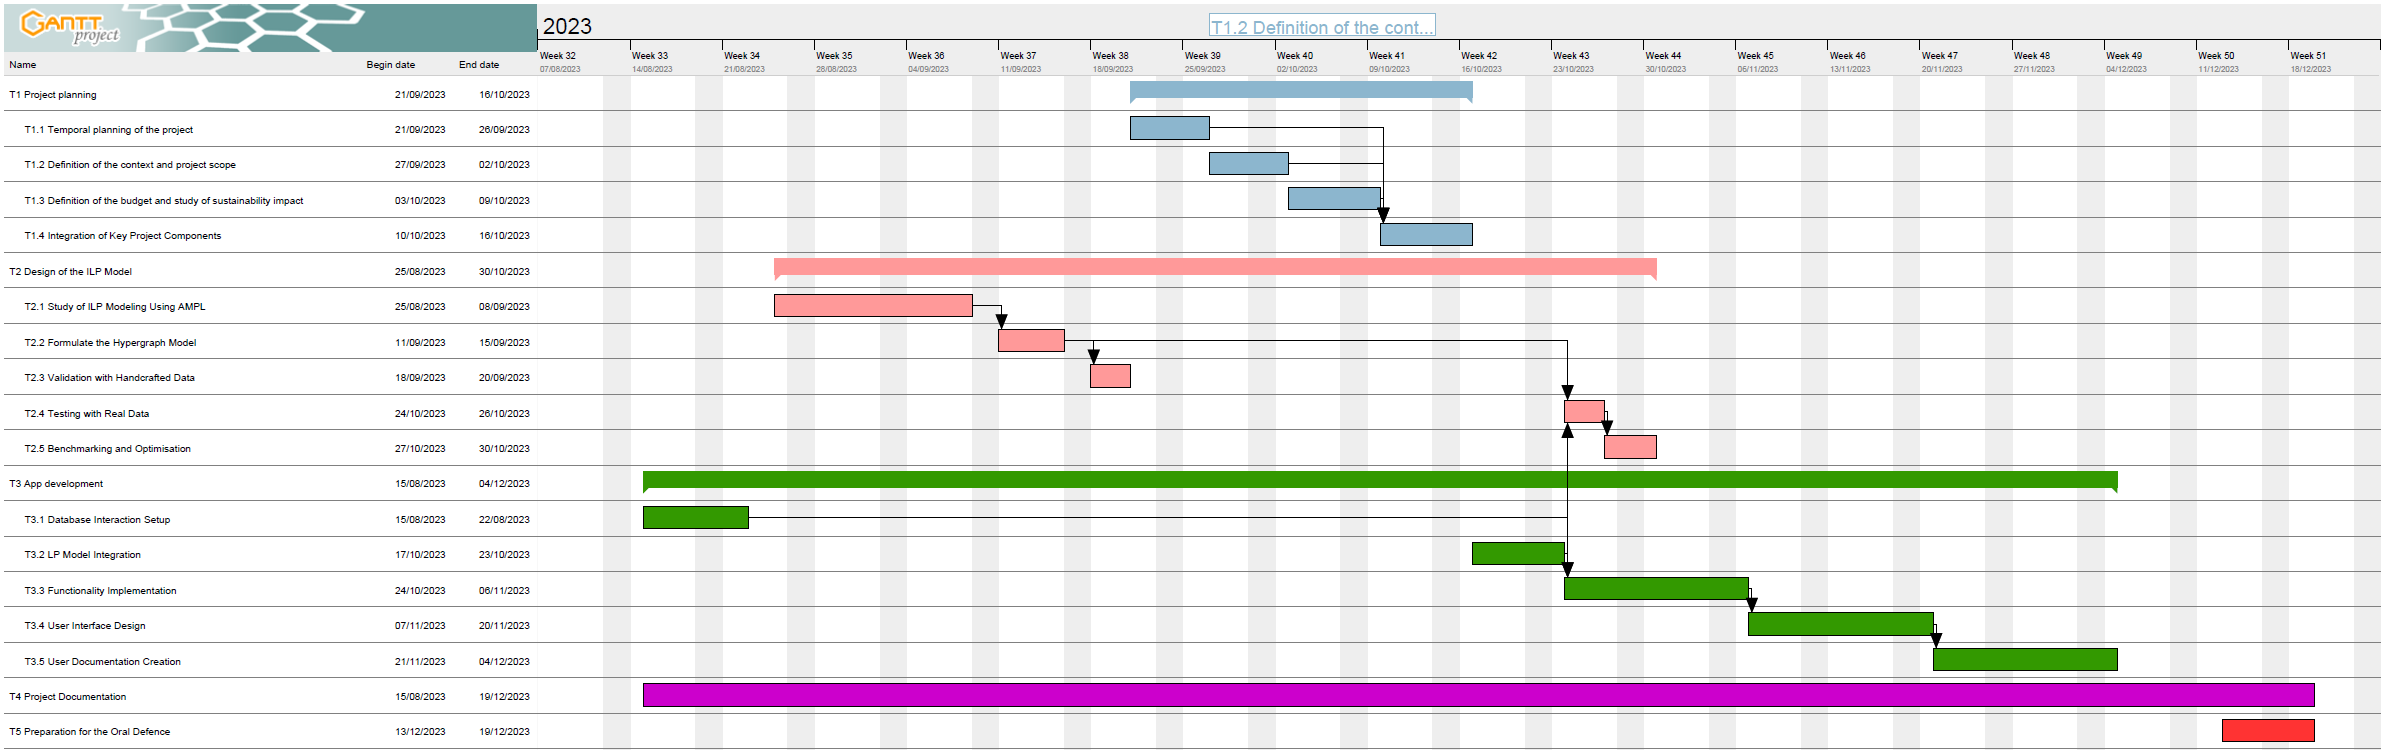
\includegraphics[scale=0.4]{GEP2/Gant.png}
  \caption{Gantt Diagram. Source : own compilation}
  \label{fig:Gantt}
\end{figure}    
\end{landscape}

\subsection{Resources}
In the pursuit of this research endeavor, several essential resources, both human and material, play a crucial role in facilitating the project's success. These resources are integral to the project's development, documentation, and overall execution.
\subsubsection{Human Resources:}
\label{sec:human_resources}
In this section, we introduce the team members working on this project and outline their roles and responsibilities:

\begin{itemize}
    \item \hypertarget{ht:author}{}\textbf{Main Developer (Author):} The principal architect of this project, the author is responsible for the project's design, development, and execution.

    \item \hypertarget{ht:supervisor}{}\textbf{University Thesis Supervisor:} The invaluable guidance and mentorship provided by the university thesis supervisor are instrumental in shaping the project's direction and ensuring academic rigor.

    \item \hypertarget{ht:GEPtutor}{}\textbf{GEP Tutor:} The GEP (GESTIÓ DE PROJECTES) tutor contributes to the project by offering instructions and feedback on the project management aspect of the research.
\end{itemize}

We have identified five distinct roles, and assigned specific responsibilities within the project:

\begin{enumerate}
    \item \textbf{Junior Project Manager:}\\
    Responsibilities: Project coordination, task scheduling, and overall project management.\\
    Assigned team member: \hyperlink{ht:author}{Author}
    \item \textbf{Project Manager:}\\
    Responsibilities: Project supervision, guidance, research leadership, methodology development, and academic oversight.\\
    Assigned team members: \hyperlink{ht:supervisor}{Thesis supervisor}, \hyperlink{ht:GEPtutor}{GEP tutor}
    \item \textbf{Junior Researcher:}\\
    Responsibilities: Research tasks, studying hypergraphs and AMPL modeling.\\
    Assigned team member: \hyperlink{ht:author}{Author}
    \item \textbf{Senior Researcher:}\\
    Responsibilities: Research and academic guidance, leadership, methodology development.\\
    Assigned team member: \hyperlink{ht:supervisor}{Thesis supervisor}
    \item \textbf{Junior Full Stack Developer:}\\
    Responsibilities: Software development, programming, and application design.\\
    Assigned team member: \hyperlink{ht:author}{Author}
\end{enumerate}

\subsubsection{Material Resources:}\label{sec:material_resources}

\hypertarget{ht:overleaf}{}\textbf{Overleaf:} A collaborative LaTeX platform, Overleaf simplifies project documentation, enabling efficient collaboration and progress tracking with the project team. \\
\hypertarget{ht:atenea}{}\textbf{Atenea:} The university's Atenea platform serves as a communication hub, providing instructions and feedback from the GEP tutor. \\
\hypertarget{ht:pycharm}{}\textbf{PyCharm IDE:} A top-tier Python Integrated Development Environment (IDE) empowers the author with advanced programming capabilities, streamlining development tasks.\\
\hypertarget{ht:chatgpt}{}\textbf{ChatGPT:} A versatile AI tool, ChatGPT assists in text composition and programming tasks, ensuring the generation of grammatically correct and comprehensive text.\\
\hypertarget{ht:amplide}{}\textbf{AMPL IDE:} The AMPL Integrated Development Environment is employed for the development and testing of AMPL (A Mathematical Programming Language) models, a critical component of the project.\\
\hypertarget{ht:github}{}\textbf{GitHub:} A robust version control platform, GitHub facilitates collaborative coding, version management, and project organization.\\
\hypertarget{ht:hpc}{}\textbf{High-Performance Computer:} Equipped with a formidable Ryzen 7 5800x3D CPU, 32GB RAM operating at 3600MHz, and an AMD Radeon RX 6900XT GPU, this high-performance computer serves as the primary development environment. In the event that this setup proves insufficient for computational demands, access to the Department of Computer Science's supercomputer cluster may be requested.

\begin{landscape}
    \begin{table}[!ht]
    \centering
    \begin{tabular}{|l|l|l|l|}
        \hline
        \rowcolor{black!25}
        ID & Task & Roles  & Material Resource \\ \hline
        \rowcolor{black!15}
        T1 & Project Management & Junior Project Manager, Project Manager & \hyperlink{ht:overleaf}{Overleaf}, \hyperlink{ht:atenea}{Atenea}, \hyperlink{ht:chatgpt}{ChatGPT}, \hyperlink{ht:hpc}{High-Performance Computer} \\ \hline
        T1.1 & Definition of the context and project scope & Junior Project Manager, Project Manager & \hyperlink{ht:overleaf}{Overleaf}, \hyperlink{ht:atenea}{Atenea}, \hyperlink{ht:chatgpt}{ChatGPT}, \hyperlink{ht:hpc}{High-Performance Computer} \\ \hline
        T1.2 & Temporal planning of the project & Junior Project Manager, Project Manager & \hyperlink{ht:overleaf}{Overleaf}, \hyperlink{ht:atenea}{Atenea}, \hyperlink{ht:chatgpt}{ChatGPT}, \hyperlink{ht:hpc}{High-Performance Computer} \\ \hline
        T1.3 & Definition of the budget and study of sustainability impact & Junior Project Manager, Project Manager & \hyperlink{ht:overleaf}{Overleaf}, \hyperlink{ht:atenea}{Atenea}, \hyperlink{ht:chatgpt}{ChatGPT}, \hyperlink{ht:hpc}{High-Performance Computer} \\ \hline
        T1.4 & Integration of Key Project Components & Junior Project Manager, Project Manager & \hyperlink{ht:overleaf}{Overleaf}, \hyperlink{ht:atenea}{Atenea}, \hyperlink{ht:chatgpt}{ChatGPT}, \hyperlink{ht:hpc}{High-Performance Computer} \\ \hline
        T1.5 & Meetings with the tutor & All roles & ~ \\ \hline
        \rowcolor{black!15}
        T2 & Design of the ILPModel & Junior Researcher & \hyperlink{ht:amplide}{AMPL IDE}, \hyperlink{ht:hpc}{High-Performance Computer} \\ \hline
        T2.1 & Study of ILP Modeling Using AMPL & Junior Researcher & ~ \\ \hline
        T2.2 & Formulate the Hypergraph Model & Junior Researcher & \hyperlink{ht:amplide}{AMPL IDE}, \hyperlink{ht:hpc}{High-Performance Computer} \\ \hline
        T2.3 & Validation with Handcrafted Data & Junior Researcher & \hyperlink{ht:amplide}{AMPL IDE}, \hyperlink{ht:hpc}{High-Performance Computer} \\ \hline
        T2.4 & Testing with Real Data & Junior Researcher & \hyperlink{ht:amplide}{AMPL IDE}, \hyperlink{ht:hpc}{High-Performance Computer} \\ \hline
        T2.5 & Benchmarking and Optimization & Junior Researcher & \hyperlink{ht:amplide}{AMPL IDE}, \hyperlink{ht:hpc}{High-Performance Computer} \\ \hline
        \rowcolor{black!15}
        T3 & App development & Junior Full Stack Developer & \hyperlink{ht:github}{GitHub}, \hyperlink{ht:pycharm}{PyCharm IDE}, \hyperlink{ht:chatgpt}{ChatGPT}, \hyperlink{ht:hpc}{High-Performance Computer} \\ \hline
        T3.1 & Database Interaction Setup & Junior Full Stack Developer & \hyperlink{ht:github}{GitHub}, \hyperlink{ht:pycharm}{PyCharm IDE}, \hyperlink{ht:chatgpt}{ChatGPT}, \hyperlink{ht:hpc}{High-Performance Computer} \\ \hline
        T3.2 & ILP Model Integration & Junior Full Stack Developer & \hyperlink{ht:github}{GitHub}, \hyperlink{ht:pycharm}{PyCharm IDE}, \hyperlink{ht:chatgpt}{ChatGPT}, \hyperlink{ht:hpc}{High-Performance Computer} \\ \hline
        T3.3 & Functionality Implementation & Junior Full Stack Developer & \hyperlink{ht:github}{GitHub}, \hyperlink{ht:pycharm}{PyCharm IDE}, \hyperlink{ht:chatgpt}{ChatGPT}, \hyperlink{ht:hpc}{High-Performance Computer} \\ \hline
        T3.4 & User Interface Design & Junior Full Stack Developer & \hyperlink{ht:github}{GitHub}, \hyperlink{ht:pycharm}{PyCharm IDE}, \hyperlink{ht:chatgpt}{ChatGPT}, \hyperlink{ht:hpc}{High-Performance Computer} \\ \hline
        T3.5 & User Documentation Creation & Junior Full Stack Developer & \hyperlink{ht:github}{GitHub}, \hyperlink{ht:pycharm}{PyCharm IDE}, \hyperlink{ht:chatgpt}{ChatGPT}, \hyperlink{ht:hpc}{High-Performance Computer} \\ \hline
        \rowcolor{black!15}
        T4 & Project documentation & Junior Full Stack Developer & \hyperlink{ht:chatgpt}{ChatGPT} \\ \hline
        \rowcolor{black!15}
        T5 & Preparation for the oral defence & Junior Researcher, Junior Full Stack Developer & \hyperlink{ht:chatgpt}{ChatGPT} \\ \hline
    \end{tabular}
    \caption{Table of requirements (Human and Material) corresponding to each task}
    \label{tab:requirementsHRMat}
\end{table}
\end{landscape}

\subsection{Risk Management: Obstacles and alternative plans}
In the pursuit of this research project, we have identified several potential risks that may affect its execution. In this section, we discuss these risks, propose solutions, and provide estimates of possible consequences in terms of additional time and resources required.\\
\subsubsection{Project Timeline}

    \textbf{Risk:} Some tasks may have been underestimated and may take longer than expected for various reasons.\\
    \textbf{Proposed Solution:} It is crucial to monitor our progress and be aware of the expected development stage at any given time. This enables us to adjust our plans if necessary.\\
    \textbf{Possible Consequences:} In the worst-case scenario, we may require an additional 50 to 80 hours of labor.\\
    \textbf{Probability:} Low. We have already conducted a comprehensive field study during the document's preparation, allowing us to identify potential obstacles and adapt the project plan and scope accordingly.
    
\subsubsection{Computational power}

    \textbf{Risk:} The computer we have may not be powerful enough to handle the largest hypergraphs efficiently.\\
    \textbf{Proposed Solution:} In case our current setup proves insufficient, we will establish contact with the computing cluster of the Department of Computer Science to process more demanding cases.\\
    \textbf{Possible Consequences:} In the event of computational limitations, there might be a delay of multiple days. During this time, Task T2.4 might be affected. However, our project plan allows us to proceed with different tasks that do not rely on T2.4 as a predecessor. At worst, we anticipate a delay of 15 hours.\\
    \textbf{Probability:} Low. Early testing shows that the computer at our dispositions is sufficiently powerful.
    
\subsubsection{Integration Challenges}

\textbf{Risk:} Integration with the KEGG database may present challenges, including content and format discrepancies.\\
\textbf{Proposed Solution:} To address integration challenges effectively, we will implement the following strategies:\\
- Stay informed about updates to the KEGG database.\\
- Establish communication channels with the KEGG team if possible.\\
- Develop a flexible application architecture capable of accommodating changes as they occur.\\
\textbf{Possible Consequences:} Integration challenges may lead to additional effort and time spent on data processing and application adaptation. The extent of the consequences will depend on the nature and frequency of changes in the KEGG database. We expect a delay of up two 50 hours.\\
\textbf{Probability:} High. We have already identified several shortcomings in the data available that could impact Tasks T3.3 and T3.4.

\subsubsection{Inexperience with ILP:}

\textbf{Risk:} The author's limited experience with Integer Linear Programming (ILP) poses a potential challenge.\\
\textbf{Proposed Solution:} To overcome inexperience with ILP, we will adopt a proactive approach that includes:\\
    - Utilizing educational resources, such as online courses and textbooks.\\
    - Seeking guidance and mentorship from experts in the field.\\
    - Engaging in practical exercises to apply ILP concepts.\\
    - Collaborating with individuals experienced in ILP.\\
    - Committing to continuous learning throughout the project.\\
\textbf{Possible Consequences:} While there may be an initial learning curve, dedicating time and effort to gaining proficiency in ILP should mitigate potential challenges related to inexperience.
Some tasks may have been underestimated and may take longer than expected for various reasons. We may expect up to extra 20 hours.\\
\textbf{Probability:} Low. We already have a working model. 


\section{Budget} \label{sec:Budget}
In this section, we present a comprehensive budget estimation for the successful completion of the project. The budget is categorized into two main components: Personnel Costs per Activity and Generic Costs. This breakdown offers transparency and insight into the allocation of resources.
\subsection{Staff costs}

As we saw in section \ref{sec:human_resources}, we identified three key individuals (the Author, the thesis supervisor and the GEP supervisor) who are involved in various roles to ensure the successful execution of the project. 

In table \ref{tab:estimatedStaffCostsPerHour}, we present the estimated hourly rates for each of the roles, taking into account Social Security contributions. The cost estimation is based on average salaries for each role in the region of Barcelona. 

\begin{table}[H]
    \centering
    \begin{tabular}{l|l|l|l}
    \rowcolor{black!15}
        Role & Annual Salary & Annual Salary + SS (35\%) & Cost Per hour \\ \hline
        Project Manager & €44,000.00 \cite{glassPM} & €59,400.00 & €34.22 \\ \hline
        Junior Project Manager & €30,000.00 \cite{glassJPM} & €40,500.00 & €23.33 \\ \hline
        Junior Researcher & €25,000.00 \cite{glassJR} & €33,750.00 & €19.44 \\ \hline
        Senior Researcher & €39,000.00 \cite{glassSR}& €52,650.00 & €30.33 \\ \hline
        Junior Full Stack Developer & €25,000.00 \cite{glassJFSD} & €33,750.00 & €19.44 \\
    \end{tabular}
    \caption{Estimated Staff Costs per hour (1736 working hours per year \cite{statistaHours})}
    \label{tab:estimatedStaffCostsPerHour}
\end{table}

In table \ref{tab:PCA}, we present the estimated cost of each task by defining how many hours each role must spend on it and by using the data from table \ref{tab:estimatedStaffCostsPerHour}. 

What we obtain is an estimation of the Personnel Cost per Activity or PCA.
\begin{landscape}
\begin{table}[!ht]
    \centering
    %\rotatebox{270}{
    \begin{tabular}{|l|l|p{1.5cm}|p{1.5cm}|l|l|p{2cm}|l|l|}
    \hline
        \multirow{2}{*}{ID} & \multirow{2}{*}{Task} & \multicolumn{5}{c|}{Hours per role} & \multirow{2}{*}{Total Hours} & \multirow{2}{*}{Price} \\\cline{3-7} 
        ~ & ~ & Project Manager & Jr.Project Manager & Jr. Researcher & Sr. researcher & Jr. Full Stack Dev. & ~ & ~ \\ \hline
        \rowcolor{black!15}
        T1 & Project Management & 25 & 75 & 5 & 10 & 5 & 120 & €3,102.82 \\ \hline
        T1.1 & Context and scope & 5 & 25 & 0 & 0 & 0 & 30 & €754.32 \\ \hline
        T1.2 & Temporal planning of the project & 5 & 15 & 0 & 0 & 0 & 20 & €521.03 \\ \hline
        T1.3 & Budget and sustainability & 5 & 15 & 0 & 0 & 0 & 20 & €521.03 \\ \hline
        T1.4 & Integration of Key Project Components & 5 & 15 & 0 & 0 & 0 & 20 & €521.03 \\ \hline
        T1.5 & Meetings with the tutor & 5 & 5 & 5 & 10 & 5 & 30 & €785.43 \\ \hline
        \rowcolor{black!15}
        T2 & Design of the ILPModel & 0 & 0 & 90 & 0 & 0 & 90 & €1,749.71 \\ \hline
        T2.1 & Study of ILP Modeling Using AMPL & 0 & 0 & 40 & 0 & 0 & 40 & €777.65 \\ \hline
        T2.2 & Formulate the Hypergraph Model & 0 & 0 & 15 & 0 & 0 & 15 & €291.62 \\ \hline
        T2.3 & Validation with Handcrafted Data & 0 & 0 & 10 & 0 & 0 & 10 & €194.41 \\ \hline
        T2.4 & Testing with Real Data & 0 & 0 & 15 & 0 & 0 & 15 & €291.62 \\ \hline
        T2.5 & Benchmarking and Optimization & 0 & 0 & 10 & 0 & 0 & 10 & €194.41 \\ \hline
        \rowcolor{black!15}
        T3 & App development & 0 & 0 & 0 & 0 & 210 & 210 & €4,082.66 \\ \hline
        T3.1 & Database Interaction Setup & 0 & 0 & 0 & 0 & 35 & 35 & €680.44 \\ \hline
        T3.2 & ILP Model Integration & 0 & 0 & 0 & 0 & 25 & 25 & €486.03 \\ \hline
        T3.3 & Functionality Implementation & 0 & 0 & 0 & 0 & 50 & 50 & €972.06 \\ \hline
        T3.4 & User Interface Design & 0 & 0 & 0 & 0 & 50 & 50 & €972.06 \\ \hline
        T3.5 & User Documentation Creation & 0 & 0 & 0 & 0 & 50 & 50 & €972.06 \\ \hline
        \rowcolor{black!15}
        T4 & Project documentation & 0 & 0 & 0 & 0 & 50 & 50 & €972.06 \\ \hline
        \rowcolor{black!15}
        T5 & Preparation for the oral defence & 0 & 0 & 15 & 0 & 15 & 30 & €583.24 \\ \hline
        \multicolumn{8}{r|}{Sum: } & €19,425.69 \\ \cline{9-9}
    \end{tabular}
    %}
    \caption{Personnel Cost per Activity (PCA) based on the costs defined in table \ref{tab:estimatedStaffCostsPerHour}}
    \label{tab:PCA}
\end{table}
\end{landscape}

\newpage

\subsection{Generic costs}
In this subsection, we examine the amortization of material resources utilized during the course of this study. Note that all the software that we use are free to use or have an free educational licence option, therefore they are not included.
To calculate the amortization of these material resources, we use the following formula:
\begin{align*}
    \text{Amortized Cost} = \frac{\text{Initial Cost}*\text{Hours of use for project}}{\text{Estimated hours of lifespan}}
\end{align*}
$\frac{}{}$
Specifically, we consider the resources in table \ref{tab:amortization}:
To calculate the values, we use :
\begin{framed}
\begin{align*}
    &\text{Hours of use for project} =& 435 \text{ hours}\\
    &\text{Estimated hours of lifespan} = &\frac{\text{Estimated years of lifespan}}{1736\text{ working hours per year} \cite{statistaHours}}
\end{align*}    
\end{framed}
\begin{table}[!ht]
    \centering
    \begin{tabular}{|l|l|l|l|}
    \hline
        \rowcolor{black!25}
        Hardware & Price & Lifetime (in years) & Amortized price \\ \hline
        Desktop Computer & €1,800 & 5 & €90 \\ \hline
        QHD VA Display & €220 & 8 & €7 \\ \hline
        Microsoft sculpt ergonomic keyboard & €80 & 5 & €4 \\ \hline
        Logitec Superlight mouse & €80 & 4 & €5 \\ \hline
        \multicolumn{3}{r|}{Total :} & €106 \\ \cline{4-4}
    \end{tabular}
    \caption{Amortization of physical resources}
    \label{tab:amortization}
\end{table}

In addition to the direct material resource costs, there are indirect expenses that need to be considered for the project. These costs are essential for the smooth operation and completion of the study.
\begin{list}{}{}
\item \textbf{Electricity}\\
   - Description: The cost of electrical consumption for running the computer, display, and other electronic equipment.\\
   - Estimated Monthly Cost: 435 hours * 0.3kW (from personal testing) * 0.1224 €/kWH \cite{priceKWH} = 15.97€

\item \textbf{Internet Service:}\\
   - Description: The cost of internet connectivity, which is crucial for research, communication, and data access.\\
   - Estimated Monthly Cost: 40€ per month \cite{priceinternet} * 12 * $\frac{435 \text{ project hours}}{8760 \text{ hours per year}}$ = 23.83€

\end{list}

\subsection{Budget Deviations}

\subsubsection{Contingency}

To account for unavoidable unexpected events, we include an additional 10\% in the total budget. This allowance is meant to accommodate the possible extra hours that may be required due to unforeseen circumstances.
We have chosen to apply the same contingency factor to both PCA and GC because they are both calculated using a linear function of the total hours used.

\subsubsection{Incidental Costs}

In the previous sections, we have identified potential risks that may emerge during the course of the project. To address these risks and mitigate their impact on the budget, we propose the inclusion of an "incidental cost" component. This allocation will serve to cover any extra expenses that may arise due to unforeseen circumstances. 

\begin{table}[!ht]
    \centering
    \begin{tabular}{|l|l|l|l|}
    \hline
    \rowcolor{black!25}
        Incident & Estimated Cost & Risk (\%) & Incidental Cost \\ \hline
        Project Timeline & €2000 & 10 & €200 \\ \hline
        Computational power & €375 & 5 & €18.75 \\ \hline
        Intergration challenges & €1250 & 50 & €625 \\ \hline
        Inexperience with ILP & €500 & 0 & €0 \\ \hline
        \multicolumn{3}{r|}{Total Incidental Cost:}& €843.75 \\ \cline{4-4}
    \end{tabular}
    \caption{Incidental Costs}
    \label{tab:incidentalCost}
\end{table}

\subsection{Management Control}
In this section, we establish essential metrics to monitor and control project expenditures, ensuring that we adhere to the original budget. Our approach involves close supervision of task durations and cost estimations per hour, allowing us to align project progress with financial expectations.

\subsubsection{Metrics for Budget Adherence:}
\begin{enumerate}
    \item \textbf{Task Duration Tracking:} We will closely monitor the actual time required to complete each task compared to the initial estimates. Deviations from estimated task durations will be identified and analyzed promptly.
    
    \item \textbf{Cost Estimation vs. Real Costs:} We will assess whether the cost estimations per hour, based on roles and responsibilities, align with actual costs incurred during the project. Any disparities will trigger further investigation.
\end{enumerate}

\subsubsection{Adaptation for Budget Control}

Adherence to the budget is paramount. In cases where metrics indicate potential budget deviations, we will take proactive measures to realign with financial expectations:

\begin{itemize}
    \item \textbf{Task Reallocation:} If certain tasks consistently exceed estimated durations, we may consider redistributing responsibilities or resources to optimize efficiency.
    
    \item \textbf{Cost Adjustments:} Should discrepancies arise between estimated and actual costs, we will evaluate the factors contributing to the variance and adjust the budget accordingly.
    
    \item \textbf{Resource Optimization:} We will explore opportunities for resource optimization, including time and material resources, to ensure efficient utilization and cost-effectiveness.
\end{itemize}

By implementing these management control measures, we aim to maintain strict budget adherence throughout the project's lifecycle. This proactive approach allows us to adapt promptly and make informed decisions to ensure financial stability and project success.

\subsection{Total Budget}
We have compiled all the budget components discussed previously into the following table \ref{tab:finalBudget} to present the overall budget for the project:
\begin{table}[!ht]
    \centering
    \begin{tabular}{|l|l|}
    \hline
    \rowcolor{black!25}
        Category & Cost\\ \hline
        PCA & €19,425.69 \\ \hline
        GC & €146.12 \\ \hline
        Incidental Cost & €843.75 \\ \hline
        \multicolumn{2}{c}{}\\ \hline
        \cellcolor{black!15}
        Total & €20,415.56 \\ \hline
        \cellcolor{black!25}
        Total with Contigency & €22,457.12 \\ \hline
    \end{tabular}
    \caption{Final Budget}
    \label{tab:finalBudget}
\end{table}

\section{Sustainability report}

The conclusion of my bachelor's program at UPC provides a valuable opportunity for self-reflection on my understanding of the environmental impact of software engineering projects.

As the author of this thesis, I acknowledge that I possess a foundational understanding of sustainability, encompassing economic, environmental, and social dimensions. However, I am committed to continuous improvement in these areas.

\subsection{Economic dimenstion}
\smalltitle{Regarding PPP: Reflection on the cost you have estimated for the completion of the project}
Reflecting on the cost estimation for this project, I find it to be a critical aspect of project planning and management. As detailed in Section \ref{sec:Budget}, we meticulously assessed the costs, factoring in personnel and material resources, to develop a comprehensive budget.

One key takeaway from this exercise is the importance of accuracy in cost estimation. By thoroughly studying the costs associated with personnel and material resources, we aimed to create a realistic budget that aligns with project goals and objectives. However, it's essential to acknowledge that cost estimates are subject to variables and uncertainties that may arise during the project's execution.
\smalltitle{Regarding Useful Life: How are currently solved economic issues (costs...) related to the problem that you want to address (state of the art)?, and How will your solution improve economic issues (costs ...) with respect other existing solutions?}
It is important to note that this is a new and unique problem. The value of the results generated by the ILP (Integer Linear Programming) model developed in this thesis is yet unknown. Unlike established research topics or methodologies, there are no existing researchers or prior studies that directly address this particular issue. Therefore, it is challenging to draw comparisons or improvements based on existing solutions.

\subsection{Environmental Dimension}
\smalltitle{Regarding PPP: Have you estimated the environmental impact of the project?}
As previously mentioned, assessing the environmental impact of this project presents a unique challenge. The value of the results derived from the ILP (Integer Linear Programming) model developed in this thesis remains uncertain, making it challenging to predict its environmental implications. In the absence of concrete data or precedents, any assessment would rely heavily on speculation.

\smalltitle{Regarding PPP: Did you plan to minimize its impact, for example, by reusing resources?}
The potential for mitigating the impact of this project, such as resource reuse, is contingent on its outcomes and applications. As previously discussed, the value and practical applications of the ILP (Integer Linear Programming) model developed in this thesis are yet to be determined. Consequently, any specific plans for minimizing impact, including resource reuse, are inherently linked to the project's findings and utilization.


\smalltitle{Regarding Useful Life: How is currently solved the problem that you want to address (state of the art)?, and how will your solution improve the environment with respect other existing solutions?}
It is important to note that this is a new and unique problem. The value of the results generated by the ILP (Integer Linear Programming) model developed in this thesis is yet unknown. Unlike established research topics or methodologies, there are no existing researchers or prior studies that directly address this particular issue. Therefore, it is challenging to draw comparisons or improvements based on existing solutions.

\subsection{Social Dimension}
\smalltitle{Regarding PPP: What do you think you will achieve -in terms of personal growth- from doing this project?}
Engaging in this project offers a unique avenue for personal growth. It will deepen my expertise in hypergraph algorithms, honing problem-solving and research skills. Navigating novel challenges will cultivate innovation and analytical thinking. Moreover, as my knowledge expands, new professional opportunities are expected to emerge, enhancing my career prospects. Managing this project independently will also refine my time management and self-discipline. In essence, this endeavor is a pivotal step in my journey of personal and professional growth.

\smalltitle{Regarding Useful Life: How is currently solved the problem that you want to address (state of the art)?, and how will your solution improve the quality of life (social dimension) with respect other existing solutions?}
It is important to note that this is a new and unique problem. The value of the results generated by the ILP (Integer Linear Programming) model developed in this thesis is yet unknown. Unlike established research topics or methodologies, there are no existing researchers or prior studies that directly address this particular issue. Therefore, it is challenging to draw comparisons or improvements based on existing solutions.
\smalltitle{Regarding Useful Life: Is there a real need for the project?}
As said previously, the value of the results generated by the ILP (Integer Linear Programming) model developed in this thesis is yet unknown.
\section{Follow up}

This section provides a detailed update on the current progress of the thesis, documented during the first two weeks of December.

\subsection{Context of the Project}

The project remains aligned with the original context, as outlined in earlier sections of this document. See section \ref{sec:context}.

\subsection{Work Plan}

The majority of the initially planned tasks progressed smoothly, with a notable exception being the integration of the KEGG database. Below is a breakdown of the original tasks as they were defined in table \ref{tab:TaskDurationAnddependencies} and an approximation of their progress.

\begin{table}[!ht]
\centering
\begin{tabular}{|l|l|l|}
\hline \rowcolor{black!25}
ID & Task & Completion \\ 
\hline
\rowcolor{black!15}
T1 & Project Management & 100\% \\\hline
T1.1 & Definition of the context and project scope & 100\%\\\hline
T1.2 & Temporal planning of the project & 100\%\\\hline
T1.3 & Budget and sustainability & 100\%\\\hline
T1.4 & Integration of Key Project Components & 100\% \\\hline
T1.5 & Meetings with the tutor & On-going\\\hline
\rowcolor{black!15}
T2 & Design of the ILP Model & 90\%\\\hline
T2.1 & Study of ILP Modeling Using AMPL & 100\% \\\hline
T2.2 & Formulate the Hypergraph Model& 100\% \\\hline
T2.3 & Validation with Handcrafted Data &  100\% \\\hline
T2.4 & Testing with Real Data &  100\%\\\hline
T2.5 & Benchmarking and Optimization &  80\%\\\hline
\rowcolor{black!15}
T3 & App development & 70\% \\\hline
T3.1 & Database Interaction Setup & 90\% \\\hline
T3.2 & ILP Model Integration & 100\% \\\hline
T3.3 & Functionality Implementation & 70\%\\\hline
T3.4 & User Interface Design & 80\%\\\hline
T3.5 & User Documentation Creation & 0\% \\\hline
\rowcolor{black!15}
T4 & Project documentation  & 50\% \\\hline
\rowcolor{black!15}
T5 & Preparation for the oral defence & 0\% \\\hline
\end{tabular}
\caption{Task Completion at follow up stage of development} 
\label{tab:TaskCompletionAtFollowUp}
\end{table}

Below is a Gantt graph representation of the work plan for the rest of the project's development.
\begin{landscape}
    \begin{figure}[H]
        \centering
        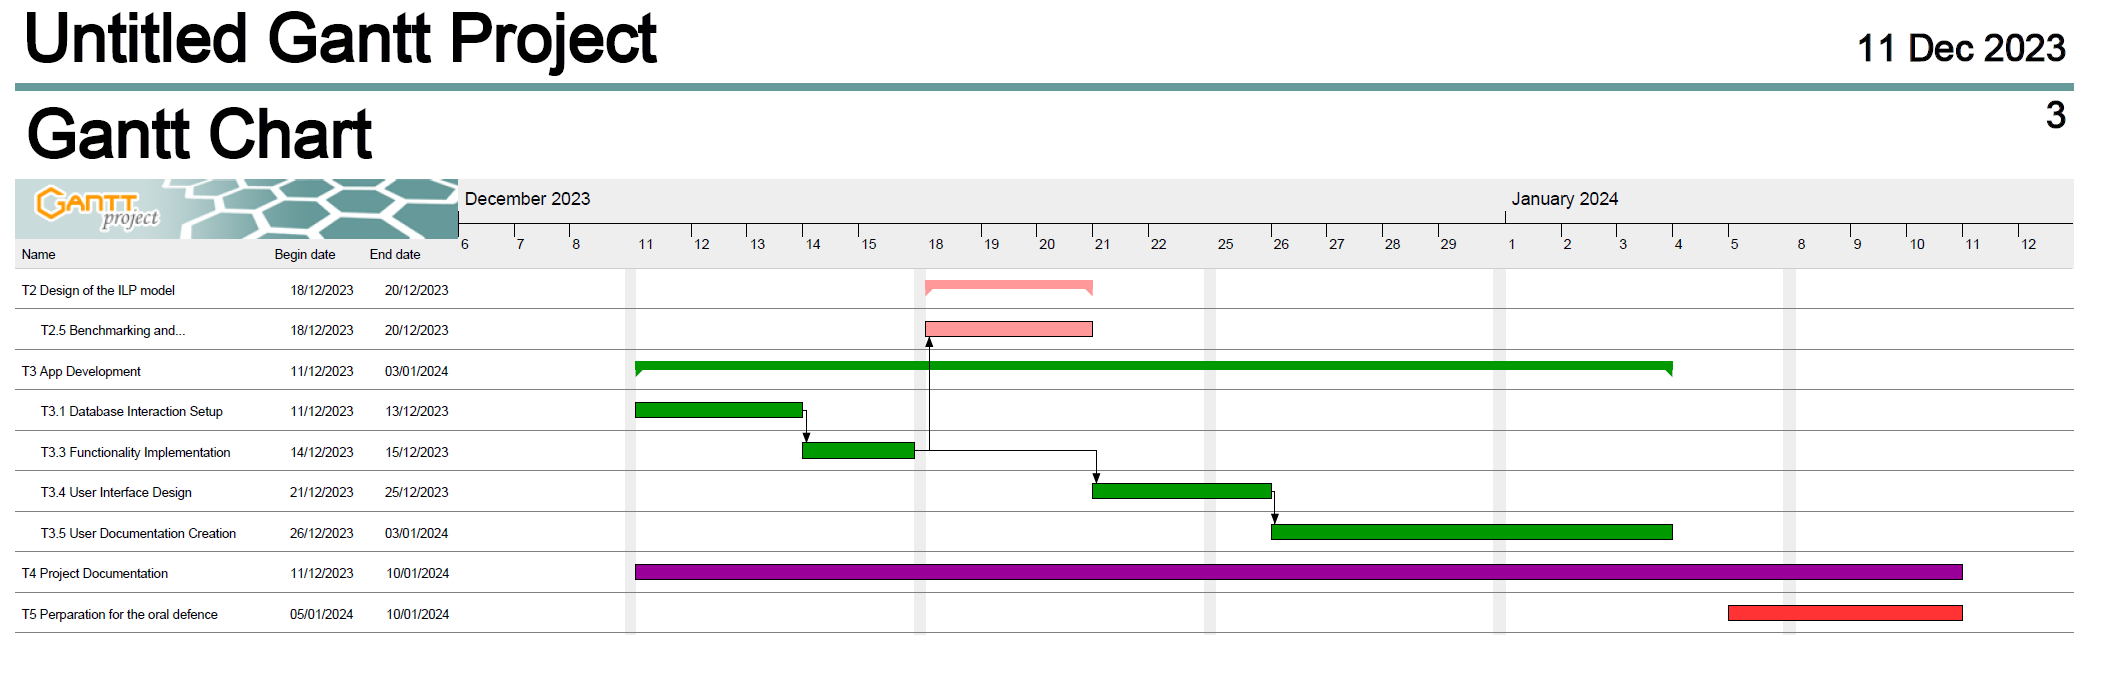
\includegraphics[scale=0.4]{Gantt2.png}
        \caption{Work plan as a Gantt Graph from 11th of december to end of project development}
        \label{fig:Gant2}
    \end{figure}
\end{landscape}

\subsubsection{Challenges in KEGG Integration}

The integration of the KEGG database posed a challenge due to the prohibitive cost of acquiring a KEGG FTP database license (USD 2,000 per academic user per year) \cite{pricelicence}.

To circumvent this financial constraint, we opted for the freely accessible KEGG REST API. In the initial approach, we aimed to query the REST API (utilizing the Python library bioservices) for each reaction, retrieving the substrates, products, and associated pathways. However, this strategy presented several drawbacks, including extended processing times and excessive request volume, leading to temporary IP bans from the KEGG Database (approximately 3 minutes for university network requests, 4 hours for private network requests).


In response to these limitations, an alternative approach was adopted, involving direct retrieval of pathway information from the KEGG database. By parsing the associated KGML files\footnote{KGML or KEGG Markup Language enables automatic drawing of KEGG pathways and provides facilities for computational analysis and modeling of protein networks and chemical networks. \cite{KGMLDescription}}, we successfully extracted reaction details. This method initially exhibited improved performance; however, we subsequently encountered omissions of substrates and products within the KGML files. To rectify this issue, we refined the strategy to extract reaction IDs from KGML files and then query the KEGG API for detailed reaction information. While this approach provided comprehensive reaction descriptions, we later discovered that the KGML files contained incomplete reaction data, omitting several reactions altogether.

Ultimately, the only viable method for obtaining a comprehensive list of reactions for a specific pathway through the REST API was to resort to the original approach of individual query-based extraction.

Despite the limitations, significant optimizations were incorporated into the final database integration to enhance efficiency.

The most significant optimization involved storing query results locally for subsequent program executions. This enhancement eliminates the need for repeated queries to the KEGG database, enabling either the utilization of persistent data (automatically downloaded from GitHub) or the on-demand rebuilding of persistent data (which can be time-consuming and require intermittent pauses in the event of IP bans). This approach ensures data accessibility while maintaining ease of use and eliminating the requirement for an active internet connection.

A further optimization involved utilizing the biopython library (BIO.KEGG.REST) to directly query the REST API, allowing us to obtain information for up to 10 reactions in one request. This significantly reduced the number of API calls required, further mitigating the risk of IP bans.

The final optimization involved introducing parallelism to the request process. By creating threads for simultaneous API queries, we could process multiple requests concurrently, further enhancing the overall efficiency of the database integration.

These optimizations collectively transformed the initial challenges into a robust and efficient database integration strategy. The optimized approach effectively balances data accuracy, computational efficiency, and user experience, enabling seamless access to KEGG metabolic pathway information.

\subsection{Methodology}

The decision to maintain the Kanban methodology as we defined it in section \ref{sec:Methodology} for the project is well-founded and aligns with the project's current trajectory and future requirements. The methodology's emphasis on visualization, limited WIP, and continuous improvement has proven invaluable in managing the project's workflow effectively and ensuring its smooth progress. As the project continues to evolve, the Kanban methodology's adaptability will provide the team with the necessary tools to navigate new challenges and maintain a high level of efficiency.

\subsection{Analysis of alternative solutions}

The problem is novel and there are currently no alternative solutions. As a matter of fact, the value of the result of the algorithm for the field of biological pathways analysis is still unclear.

\subsection{Integration of knowledge}
The project's success lies in its ability to seamlessly integrate knowledge from various disciplines, including integer linear programming, parallelism and user interface design. By drawing upon these diverse perspectives, we were able to develop a comprehensive understanding of the problem and identify potential solutions that transcended the limitations of any single discipline.

\subsection{Identification of applicable laws and regulations}

The data for this thesis was obtained from the publicly accessible KEGG REST API, and the code was developed solely by the thesis team using GitHub Copilot, ensuring compliance with all applicable data and copyright regulations.

\newpage
%\bibliographystyle{acm}
\bibliographystyle{unsrt}
\bibliography{sample}

\end{document}